% npj Digital Medicine: the Discussion admits no subheadings and no
% separate limitations or conclusions sections. The content below is the
% same as the subheaded version kept in
% 04_discussion_SUBHEADED_backup.tex.bak, rewritten as continuous prose.
\section*{Discussion}

Computational pathology has converged on a single output for
mutation prediction: a probability per gene.
The implicit assumption is that this probability is comparable
across genes and that improvement on the cohort-mean metric is
the figure of merit.
Our results challenge both assumptions.
The same cohort, same encoder, same MIL backbone yields
qualitatively different gene-level behaviour: encoder
saturation on TP53/EGFR (where additional pattern information
adds nothing), inter-pattern co-occurrence on KRAS (where only
a non-additive aggregator captures the IMA proxy), and an
unusable pattern channel on STK11/KEAP1/RBM10---out-of-ontology
for the first two, whose signal lives in stromal or biochemical
substrates the 6-pattern ontology does not encode, but merely
unestimable for RBM10, whose pattern-side atoms are demonstrably
non-empty at $n_+\!=\!37$.
The Conclusive/Inconclusive flag we report alongside each AUROC
is therefore not a cosmetic addition---it is a statement that
the cohort-level metric does \emph{not} translate uniformly into
per-slide actionability, and that downstream clinical use must
be gene-conditional.

Reading the results gene-conditionally also changes what counts as
the contribution.
The pattern-informed channel does not win the cohort-mean
benchmark---the upper tier of \cref{tab:mutation_luad_resultssec}
is statistically tied within $\pm 0.02$ AUROC.
What pattern-informed MIL does win is the \emph{argument} with the
pathologist.
A model that says ``P(KRAS) = 0.965 because the
lepidic$\,\times\,$solid Choquet interaction is $+0.032$ on the
top-200 attended tiles'' invites a textbook reply about the
invasive mucinous adenocarcinoma proxy.
A model that instead reports $P(\text{KEAP1}) = 0.610$ with a
negligible Choquet interaction and a SHAP/ablation split that places
almost all of the slide-level signal in the embedding channel and
essentially none in the pattern channel
(\cref{tab:pid_regimes}, with the exact figures in Results) is honest
about what the slide cannot answer, and points the next investigation
toward NRF2 immunostaining or RNA-seq rather than another loss
function.
This is the central clinical claim of the paper: \emph{when the
predictor is wrong, the explanation is most valuable}, and only a
pattern-informed pipeline gives the explanation a vocabulary the
pathologist can act on.\cite{rudin2019stop,holzinger2019causability}

Read through the translation lens introduced above, our results
belong to a well-established family of medical machine-learning
tasks in which one clinically inexpensive or ubiquitous modality is
mapped onto a second, more costly or latent one, with a
faithfulness that is bounded by how much of the target signal the
source physically encodes.
Placing our LUAD map beside these tasks clarifies both what is and
what is not surprising about the per-gene ceiling
(\cref{fig:fidelity_spectrum}).
The family runs from virtual staining, the literal image-to-image
case in which tissue autofluorescence is translated into stained
histology at pathologist-level fidelity precisely because the source
physically contains the target\cite{rivenson2019virtualstaining},
through ECG-to-function mapping, where an electrical modality
faithfully encodes a structural one ($\mathrm{EF}\!\leq\!35\%$,
$\auroc=0.93$)\cite{attia2019ecg}, and retinal-to-systemic mapping,
which recovers cardiovascular risk factors from fundus photographs
and so surfaces signal not previously thought to be morphologically
encoded\cite{poplin2018retinal}, to pathomics-to-genomics on the
very H\&E substrate we use\cite{kather2019msi,kather2020pancancer}.
Radiogenomics is the most instructive of them, because it already
exhibits the phenomenon we formalise: IDH and 1p/19q are recovered
at high accuracy while MGMT-promoter methylation translates markedly
less well\cite{chang2018radiogenomics}---a \emph{per-marker} split
of the same kind as our per-gene regimes.

\begin{figure}[ht!]
  \centering
  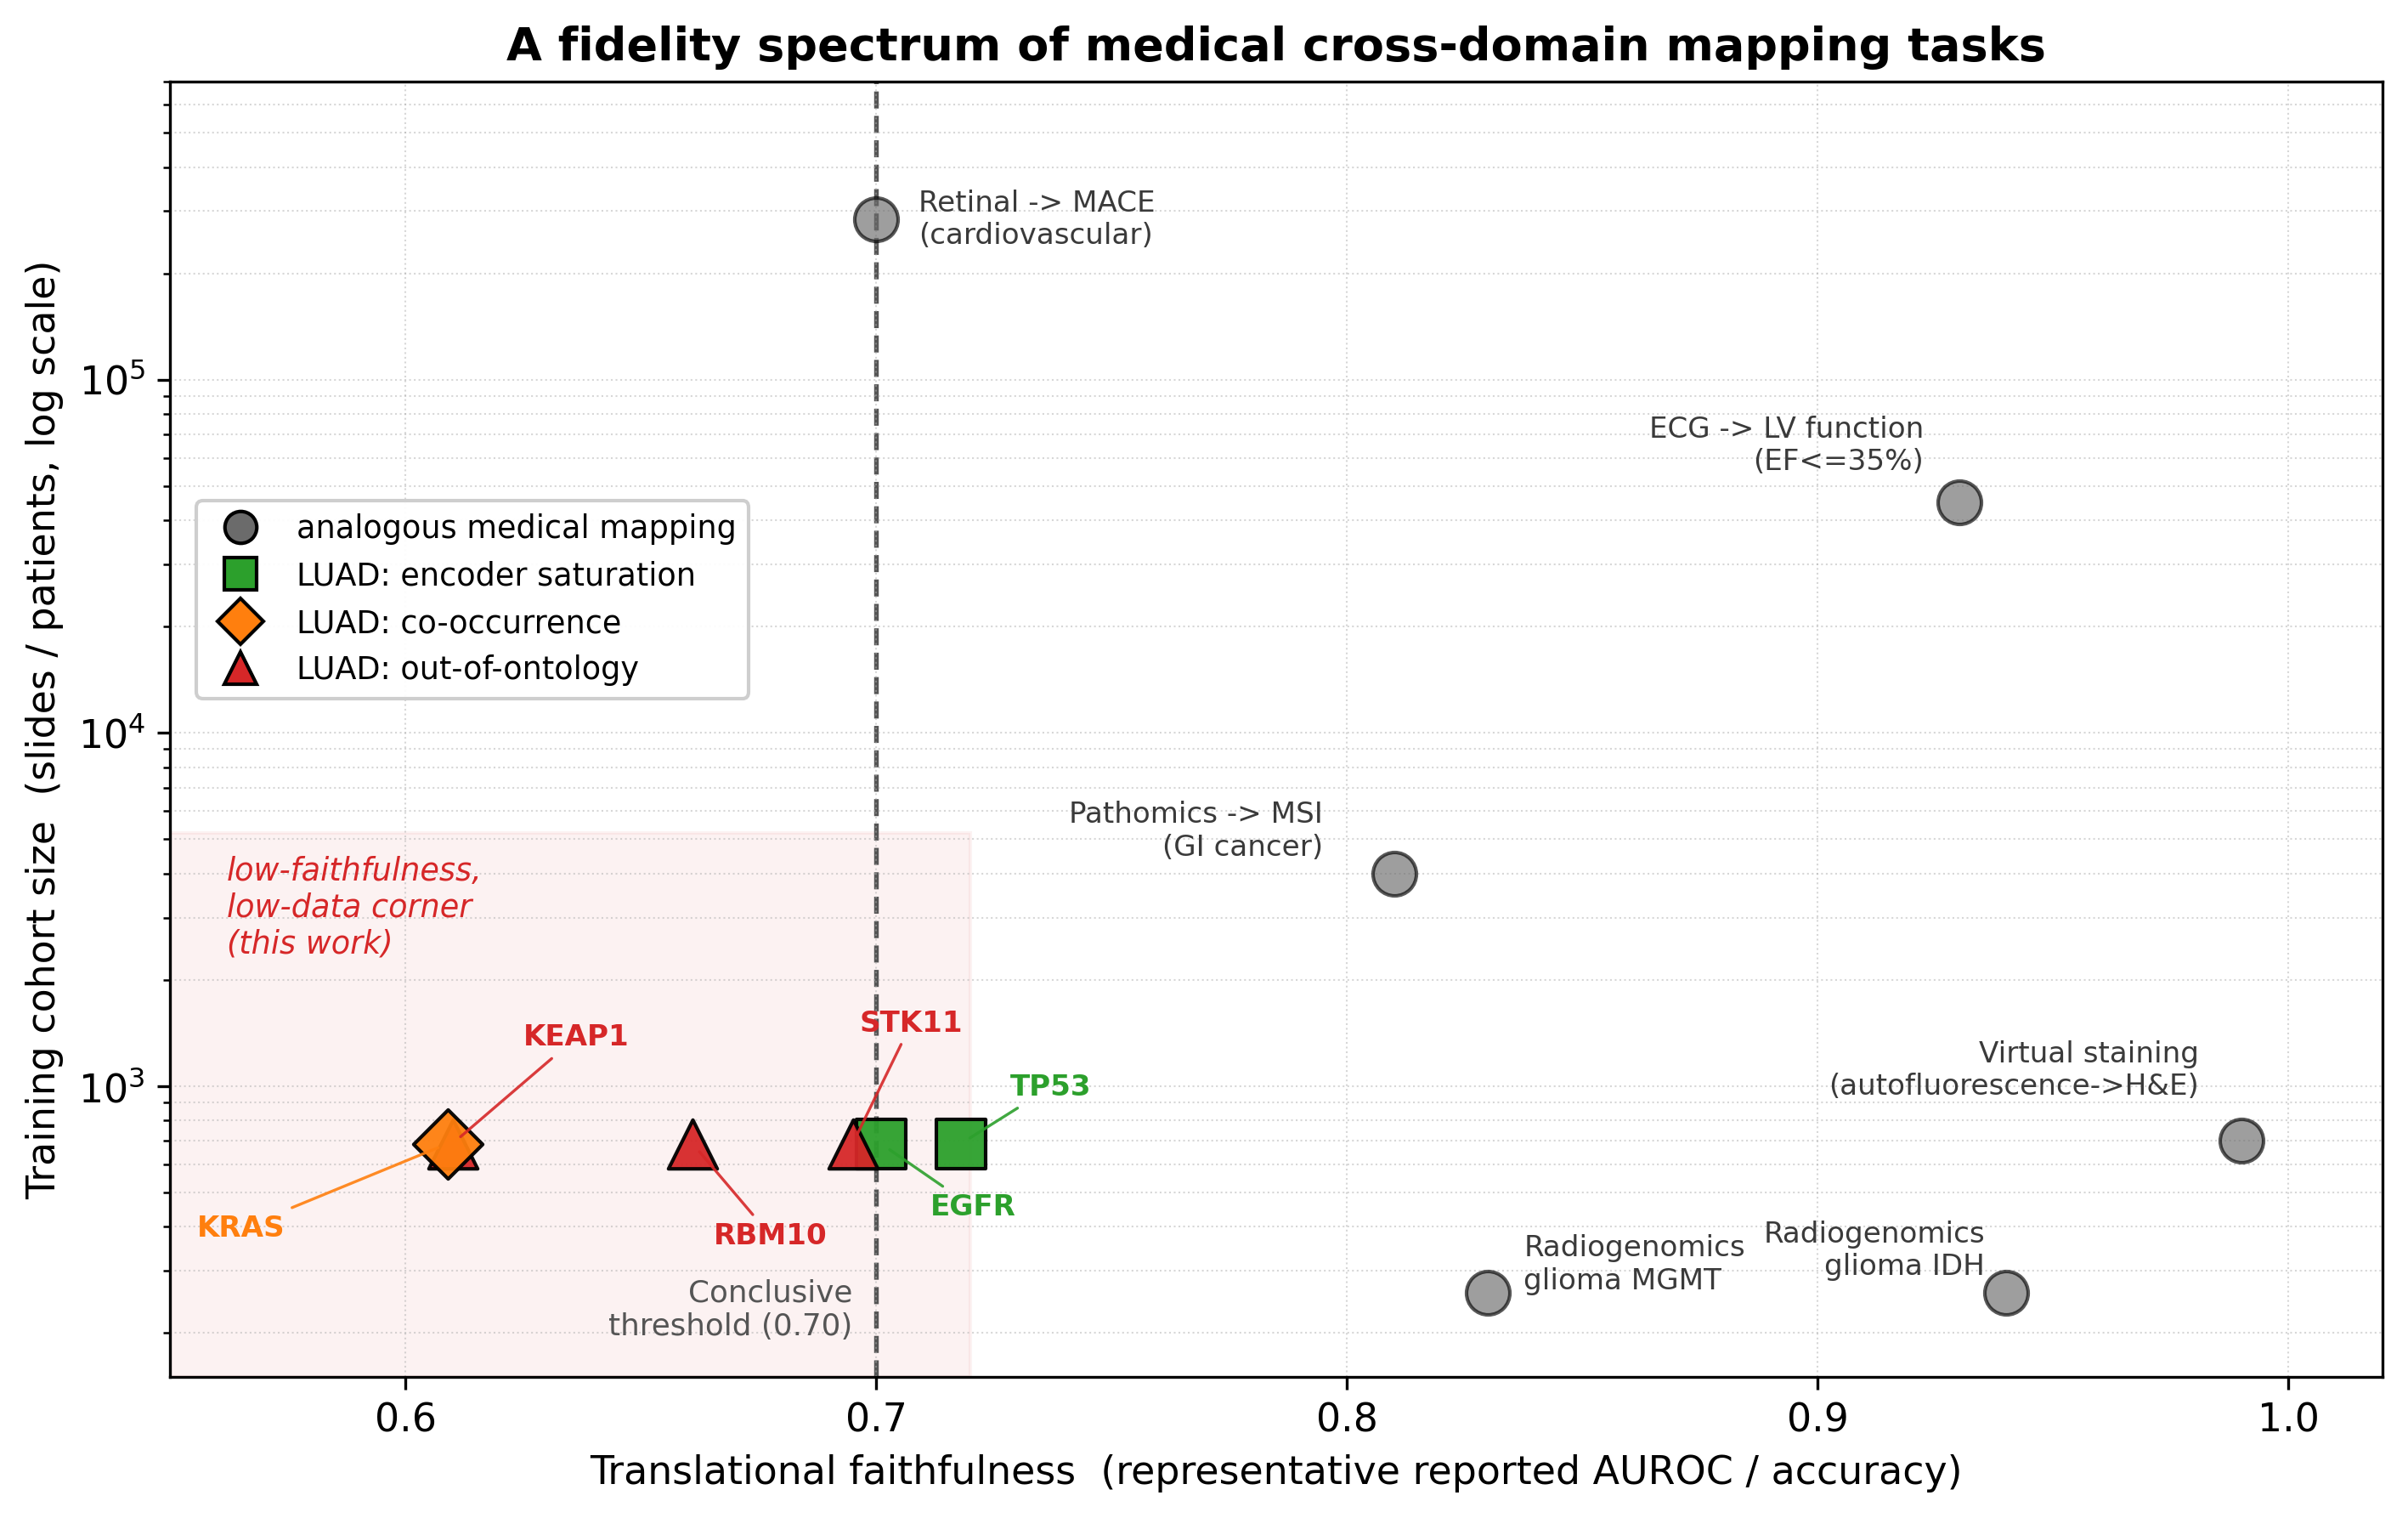
\includegraphics[width=\linewidth]{fidelity_spectrum}
  \caption{\textbf{A fidelity spectrum of medical cross-domain mapping
tasks.} Each task maps an inexpensive or ubiquitous source modality
onto a more costly or latent target; the horizontal axis is the
  representative reported AUROC/accuracy (translational faithfulness)
  and the vertical axis the training-cohort size (log scale).
  Analogous tasks span virtual staining (near-perfect, source
  physically contains
  target)\cite{rivenson2019virtualstaining}, ECG-to-left-ventricular
  function\cite{attia2019ecg}, radiogenomics of
  glioma\cite{chang2018radiogenomics},
  pathomics-to-microsatellite-instability\cite{kather2019msi} and
  retinal-to-cardiovascular mapping\cite{poplin2018retinal}. The six
  LUAD genes of this work occupy the \emph{low-faithfulness,
  low-data} corner (shaded); the dashed line is the Conclusive
  verdict threshold (AUROC $0.70$). Marker shape encodes the
  three-regime taxonomy.}
  \label{fig:fidelity_spectrum}
\end{figure}

Against this backdrop our LUAD map sits at the
\emph{low-faithfulness, low-data} corner
(\cref{fig:fidelity_spectrum}; per-gene
$\auroc\in[0.6,0.72]$; positive sets down to $n_+\!=\!37$ for
RBM10).
The three-regime taxonomy is the diagnostic that explains
\emph{why} a given gene lands there---encoder saturation, a missing
non-additive grammar, or genuine out-of-ontology
untranslatability---and therefore whether the remedy is a better
translator (architecture), a richer source vocabulary
(micro-environment channels) or a different source modality
altogether (RNA-seq, radiology).
The recurring lesson across all of these tasks is the one our
Conclusive/Inconclusive verdict operationalises: the value of a
cross-domain map is set by the physics of the source, not by the
sophistication of the estimator, and transparent per-target
reporting of that ceiling is what turns the map into a usable
clinical tool.

What lifts this from an empirical grouping to a portable claim is
that the regimes are not a grouping at all.
A taxonomy that merely groups genes by their AUROC is a description
of one cohort and travels no further than that cohort.
The three regimes are instead a decomposition: the pattern channel
and the embedding channel are two sources of information about the
same target, and \cref{eq:pid} states the only four ways that
information can be distributed between them
(\cref{tab:pid_regimes}).\cite{williams2010pid,bertschinger2014unique}
Once stated this way, the taxonomy makes commitments that can be
checked, and the check reported in Results---that the non-additive
aggregator wins on exactly the genes with a recoverable synergistic
atom and loses elsewhere---is the kind of evidence a leaderboard
comparison cannot produce.

The specific bridge we draw is between the $2$-additive Choquet
interaction index and the synergistic atom.
These are objects of different kinds: $I_{jk}$ is a learnable,
differentiable, per-slide parameter of an aggregation operator,
whereas $\Isyn$ is a property of a joint distribution that is
notoriously hard to estimate in high dimension.
The correspondence we establish is one of sign and support---a
supra-additive fuzzy measure on a pattern pair is the aggregator's
way of paying for joint activation, which is what a positive
synergistic atom licenses---and it is what makes the atom
inspectable at the bedside rather than only in a contingency table.
We do not claim that $I_{jk}$ is a consistent estimator of
$\Isyn$; establishing the conditions under which it is, or bounding
the gap, is the natural theoretical continuation of this work.

The practical consequence is a change in how the field should
decide what to build next.
Under a cohort-mean metric, the question ``what should we add?''
has one answer for all genes and it is usually more parameters or
more slides.
Under \cref{eq:pid} the question is atom-conditional: a redundant
atom means no aggregator change will help and the encoder is the
binding constraint; a synergistic atom means the aggregator's
hypothesis space is the binding constraint; an empty pattern-side
atom means the \emph{source vocabulary} is the binding constraint
and only a new channel will move it.

The translation frame does more than organise the results; it
suggests a different stance on interpretability itself.
Mainstream explainable-AI methods for computational pathology are
\emph{post-hoc and attributive}: a saliency map, an attention
overlay or a SHAP value indicates \emph{where} in the slide the
model attended, but not in a vocabulary the pathologist can contest
line by line.\cite{rudin2019stop,jain2019attention}
Reading the pipeline as a translator reframes explanation as the
act of \emph{exhibiting the translation}: the six-level stack (C2)
is a bilingual dictionary that must express every prediction in the
source language of growth patterns (L2), expose the non-additive
\emph{grammar} that couples them (L4 Choquet--Shapley interactions),
and hand the result to a target-domain lexicon (the NCIt$+$MONDO
knowledge graph, C4) that forbids invented genotype terms.
Interpretability becomes contrastive and bilingual rather than a
heat-coloured monologue.

The sharper consequence is that \emph{untranslatability is promoted
to a first-class, actionable result}---provided it is asserted at the
level where it was established.
This is the qualification we most want to press, because the
temptation the framework creates is precisely to skip it.
The Conclusive/Inconclusive verdict thresholds a mean \auroc{}, a
property of the cohort and not of any slide, so reading a low cohort
mean as ``this mutation cannot be seen in this tissue'' is a level
error---and a costly one, because it discards exactly the cases
where the morphology \emph{does} speak.
KRAS is our counterexample and it is unambiguous
(\cref{fig:kras_lepidic_solid_proxy}): a gene that is Inconclusive as
a population ($\auroc = 0.609$) yet carries confident,
tissue-localised per-slide calls wherever the IMA-associated
lepidic$\times$solid morphology is present.
Nothing about those slides is untranslatable.
What is true is that the subpopulation in which the translation holds
is a minority of the cohort, so the average over case pairs is
mediocre---a statement about population heterogeneity, not about the
expressive capacity of the source modality.

Untranslatability proper is therefore a narrower and stronger claim:
that the source-side atoms of \cref{eq:pid} are empty at the level
being discussed.
When a gene meets it, the honest output is not a low probability
presented as if it were a confident call, but the statement that the
mutation cannot be said in morphological words---and, via the
per-slide channel ablation (L5) and the SHAP embedding/pattern split
(L3), \emph{why}: the signal is in the immune micro-environment
(STK11) or in a biochemical axis with no H\&E correlate (KEAP1).
A translation that returns ``this sentence has no equivalent in the
target language, and here is the missing vocabulary'' is more useful
to the next experiment---NRF2 immunostaining, TIL quantification,
RNA-seq---than a fluent but ungrounded paraphrase, and it is the
decomposition that makes the statement specific enough to act on:
the three states an Inconclusive verdict can hide
(\cref{tab:pid_regimes}) share a mediocre AUROC while calling for
different experiments.
We therefore position the Conclusive/Inconclusive verdict as a
population-level translatability flag rather than as a per-case
confidence threshold or as a verdict on the modality, and we argue
that reporting untranslatability explicitly---with its level
attached---is a distinct and underused mode of interpretability for
cross-domain medical prediction.

A framework that has only ever been run on the cohort it was designed
around is indistinguishable from a description of that cohort.
The decomposition of \cref{eq:pid} needs exactly two ingredients---an
expert-defined controlled vocabulary on the source modality and a
learned encoder of that modality unconstrained by the
vocabulary---and both are available in domains far from pathology.
We therefore pre-register two instantiations on fully public data
(\cref{tab:crossdomain_protocol}), specified here so that the
framework can be falsified independently of the LUAD results.

\begin{table}[h!]
\centering
% Table tab:crossdomain_protocol — the framework instantiated in three domains.
% Column 1 = framework element; columns 2-4 = its realisation per domain.
% Domain A (LUAD) is reported in this paper; B and C are external validations,
% largely measured (glioma IDH/1p19q pilot + MGMT at full power, ECG sex/age)
% and partly predicted (ECG lab/structural-heart targets).
\footnotesize
\setlength{\tabcolsep}{4pt}
\renewcommand{\arraystretch}{1.15}
\begin{tabularx}{\linewidth}{l X X X}
\toprule
\textbf{Framework element} &
  \textbf{A. LUAD (this paper)} &
  \textbf{B. Glioma (external)} &
  \textbf{C. ECG (external)} \\
\midrule
Source modality
  & H\&E whole-slide image
  & Preoperative multiparametric MRI
  & 12-lead electrocardiogram \\
Target domain
  & 6 somatic driver mutations
  & IDH, 1p/19q, MGMT
  & Physiological state (sex, age; measured here). Laboratory
    abnormalities and structural heart disease remain predicted \\
\midrule
Source ontology
  & ANORAK, 6 growth patterns\cite{anorak2024}
  & VASARI, $\sim$30 semantic MR features\cite{gutman2013vasari,vasari_tcia}
  & SCP-ECG, 71 statements (44 diagnostic, 19 form, 12
    rhythm)\cite{wagner2020ptbxl} \\
Ontology already graded?
  & No; fuzzy membership learned
  & No; ordinal expert scores
  & \textbf{Yes}: $0$--$100$ likelihood per statement, native to L6 \\
Vocabulary renderer
  & \fuzzyarc{}\,V2 on Zenodo-ANORAK ($n=637$ tiles)
  & VASARI-feature classifier on the TCIA-annotated seed
    ($n=178$ LGG and $75$ GBM scored; $63$ LGG carry the matched MRI
    and molecular call the protocol needs)
  & Direct: statements are supplied per record \\
Propagated to
  & 687 TCGA-LUAD slides
  & $\sim$1{,}251 BraTS 2021 subjects\cite{baid2021brats}
  & 21{,}799 PTB-XL records; MIMIC-IV-ECG\cite{gow2023mimicivecg} \\
Target lexicon (KG)
  & NCIt $+$ MONDO
  & NCIt $+$ MONDO $+$ RadLex
  & SNOMED-CT, supplied pre-mapped\cite{strodthoff2023ptbxlplus} \\
\midrule
Regime (i) saturation
  & TP53, EGFR
  & IDH ($\auroc\!\approx\!0.88$\cite{chang2018radiogenomics};
    v1 pilot $0.90$)
  & \textbf{Sex} ($0.90$) and \textbf{age}$\,\geq\!65$ ($0.84$), both
    measured (\cref{tab:ecg_domainc}); NT-proBNP
    ($\auroc\!\approx\!0.78$) as reported by\cite{xiao2025anyecglab},
    not run here \\
Regime (ii) co-occurrence
  & KRAS (lepidic$\times$solid; non-additive ii-b)
  & 1p/19q (additive ii-a, $0.74$ by concat fusion; non-additive deferred)
  & Not populated by the two measured targets; candidate pairs for the
    predicted ones, e.g.\ LVH$\times$strain \\
Regime (iii) out-of-ontology
  & STK11, KEAP1 (RBM10: estimation floor)
  & \textbf{MGMT} (full BraTS cohort $n\!=\!577$: every condition at chance,
    $\auroc\!\approx\!0.53$--$0.56$, Inconclusive; matches the published
    $0.50$--$0.56$)\cite{kim2022mgmtvalidation,robinet2023mgmt,saeed2023mgmt}
  & Not populated by the two measured targets; troponin~I
    ($\auroc<0.55$) and $16$ of $108$ targets as reported
    by\cite{xiao2025anyecglab}, not run here \\
\midrule
Falsification test
  & Non-additive aggregator wins on regime-(ii-b) targets only
  & Additive fusion recovers 1p/19q but not IDH or MGMT (MGMT at chance
    in all conditions); the non-additive ii-b read on 1p/19q awaits a
    larger cohort
  & Non-additive aggregator wins only where a statement pair interacts:
    on sex and age no pair does
    ($\lvert\mathrm{FC}\!-\!\mathrm{PI}\rvert\!\leq\!0.002$) and both
    stay in regime~(i) \\
Access
  & GDC, public
  & TCIA/IDC $+$ BraTS 2021, public
  & PhysioNet, open (PTB-XL, PTB-XL+, MIMIC-IV-ECG) \\
\bottomrule
\end{tabularx}
\begin{flushleft}\footnotesize
The framework requires only an expert source vocabulary and an
unconstrained learned encoder of the same modality; every row above
is an instance of the same decomposition, not an analogy.
Domain~B is chosen because MGMT is the best-documented
population-level translation failure in the field and is currently
reported as a defeat rather than as a result; scored here at full power
($n\!=\!577$) it is Inconclusive in every condition
(\cref{tab:glioma_domainb}), so the framework issues that decade-old
failure as a diagnostic verdict. The strict separation of
untranslatability from a diluted subpopulation effect
(\cref{tab:levels_of_analysis}) is limited by the propagated---rather than
expert-scored---VASARI channel and rests on the encoder remaining at chance.
Domain~C is chosen because its source ontology is
already graded and ontology-mapped. The two targets scored here---sex
and age---are physiological rather than laboratory ones, and they test
that the four-condition protocol and the verdict survive a change of
modality family. The $108$ laboratory indicators the domain also
affords would test whether the taxonomy scales beyond six targets;
that question is posed by the literature cited in the regime rows and
is not settled by this run.
\end{flushleft}

\caption{The translatability framework instantiated in three domains.
Domain~A is reported in this paper; domains~B and~C are
pre-registered, with data sources, source ontologies and the expected
regime assignment fixed in advance.}
\label{tab:crossdomain_protocol}
\end{table}

The level structure of \cref{tab:levels_of_analysis} transfers with
the framework. In every domain the source channels are defined on a
single \emph{unit}---a slide in LUAD, a scan in glioma, a record in
ECG---but the \pid{} atoms of \cref{eq:pid} and the
Conclusive/Inconclusive verdict of \cref{eq:conclusive_verdict} are
expectations over the joint distribution of those channels and the
label, and are therefore \emph{population}-level in all three cases;
probability and the L1--L6 interpretability instruments remain
per-unit (\cref{tab:levels_crossdomain}). Two consequences follow.
First, the population-level synergistic atom $\mathcal{S}$ has a
per-unit counterpart in the Choquet interaction index $I_{jk}$, so
regime~(ii) is falsifiable at both levels in each domain---between
growth patterns on a slide, between VASARI features on a scan, and
between SCP-ECG statements on a record. Second, an Inconclusive
population verdict is compatible with the same three states of the
world in every domain (information absent at every level; present in a
morphologically or radiologically defined subpopulation and diluted in
the average; or present but unestimable at the available positive-set
size), so the per-stratum readout we use to adjudicate KRAS here is the
same instrument that separates strict MGMT untranslatability from a
diluted VASARI stratum in domain~B. The only structural difference is
that a slide and a scan are \emph{bags} aggregated by MIL, whereas an
ECG record is a \emph{single instance}: its sub-unit level collapses
and synergy is read between vocabulary statements directly.

\begin{table}[h!]
\centering
% Table tab:levels_crossdomain — the level structure of tab:levels_of_analysis
% generalised to the three domains. The point is that the PID atoms and the
% Conclusive/Inconclusive verdict are population-level in every domain, while
% probability and the interpretability instruments are per-unit; only the name
% of the unit (slide -> scan -> record) and whether it is a bag or a single
% instance change across domains.
\footnotesize
\setlength{\tabcolsep}{4pt}
\renewcommand{\arraystretch}{1.15}
\begin{tabularx}{\linewidth}{>{\raggedright\arraybackslash}p{3.0cm} X X X}
\toprule
\textbf{Level (quantities estimated here)} &
  \textbf{A. LUAD} &
  \textbf{B. Glioma} &
  \textbf{C. ECG} \\
\midrule
\textbf{Population} \newline mean $\auroc$, the \pid{} atoms of
  \cref{eq:pid}, regime assignment, and the verdict of
  \cref{eq:conclusive_verdict}
  & target $\times$ cohort; 6 mutations over 668 patients
  & target $\times$ cohort; IDH, 1p/19q, MGMT
  & target $\times$ cohort; 108 laboratory indicators $+$ 12 SHD \\
\midrule
\textbf{Patient} \newline label; fold membership; $P(\cdot)$ pooled
  over that patient's units
  & patient (668)
  & subject ($\sim$1{,}251)
  & patient (18{,}869) \\
\midrule
\textbf{Unit} \newline per-unit $P(\cdot)$; the L1--L6 stack;
  Choquet--Shapley $\Phi_k$ and interaction indices $I_{jk}$
  & WSI slide (687); \emph{bag} of tiles
  & MRI scan ($\sim$1{,}251); \emph{bag} of slices/patches
  & ECG record (21{,}799); \emph{single instance} \\
\midrule
\textbf{Sub-unit} \newline local evidence; where in the signal it sits
  & tile $224\!\times\!224$ px ($\leq\!200$/slide)
  & slice / patch
  & --- collapses (optional: beat / lead) \\
\bottomrule
\end{tabularx}
\begin{flushleft}\footnotesize
Every row is the same object renamed, not an analogy. The \pid{} atoms
and the Conclusive/Inconclusive verdict are \emph{population}-level in
all three domains---they are expectations over the joint distribution
of the source channels and the label, so a single unit cannot carry
them---while probability and the interpretability instruments are
\emph{per-unit}. The synergistic atom $\mathcal{S}$ of \cref{eq:pid}
(population) has its per-unit counterpart in the Choquet interaction
index $I_{jk}$, which is why the non-additive sub-form (ii-b) of
regime~(ii) is testable at both levels.
The only structural difference is that in A and B the unit is a
\emph{bag} (MIL aggregation over sub-units), whereas an ECG record is a
\emph{single instance}: the sub-unit level collapses, and synergy is
read between vocabulary statements (e.g.\ LVH$\times$strain) rather than
between sub-unit patterns.
\end{flushleft}

\caption{The level structure of \cref{tab:levels_of_analysis}
generalised to the three domains. The population level hosts the \pid{}
decomposition and the verdict in every domain; the interpretability
instruments are per-unit. Only the name of the unit and whether it is a
bag or a single instance change across domains.}
\label{tab:levels_crossdomain}
\end{table}

The first instantiation, glioma MRI $\rightarrow$ genotype, is the
closest structural analogue: an image of a tumour mapped
onto its molecular profile, on open data, with an expert vocabulary
already in place.
VASARI is a consensus-defined controlled terminology of roughly
thirty semantic MR features---enhancement quality, necrosis, margin
definition, oedema, ependymal contact, grey-level
heterogeneity---published with per-subject scores and reported
inter-observer agreement for the TCGA glioma
collections.\cite{gutman2013vasari,vasari_tcia}
The transfer of our pipeline is one-to-one: a VASARI-feature
classifier trained on the TCIA-annotated subset ($n=178$ LGG,
$n=75$ GBM) and propagated to the $\sim$1{,}251 BraTS 2021
subjects\cite{baid2021brats} occupies the position that
\fuzzyarc{}\,V2 trained on Zenodo-ANORAK and propagated to TCGA-LUAD
occupies here, with the same 2-additive Choquet aggregator over the
feature vector.

What makes this domain worth the effort is the target, not the
method.
MGMT promoter methylation has resisted prediction from preoperative
MRI for a decade: the BraTS 2021 radiogenomic challenge was won at
$\auroc\!\approx\!0.62$ on its own validation split, but subsequent
CNN, ViT and Swin variants evaluated externally collapse to chance
($\auroc\!\approx\!0.50$--$0.56$),\cite{baid2021brats,saeed2023mgmt} a systematic
re-evaluation concluded that the algorithms developed to date are
``not suitable for clinical application'',\cite{robinet2023mgmt} and
an external validation across $985$ patients concluded that the
methylation status ``may not be predictable'' from conventional
structural MRI even with deep
learning.\cite{kim2022mgmtvalidation}
That literature is, in our terms, a decade of accumulating evidence
for a regime-(iii) verdict---reported as a community-wide defeat
because no framework existed in which it could be reported as a
finding.
Our prediction is specific and falsifiable: IDH should sit in
regime~(i) with the VASARI channel adding nothing on top of the
encoder; 1p/19q should sit in regime~(ii), with the non-additive
aggregator beating the additive one on that target \emph{and on no
other}; and MGMT should sit in regime~(iii) with empty
VASARI-side atoms.
That last prediction is the strong one, because it asserts the
strict form of untranslatability and therefore has to exclude the
two weaker states that produce the same stalled AUROC: a data floor,
which the $n\!\sim\!1{,}251$ BraTS cohort makes implausible, and a
subpopulation effect of the kind KRAS exhibits here, which is
excluded only if no VASARI-defined stratum recovers the signal.
We will report the per-stratum readout for exactly that reason.
If the strict form holds, the remedy is a different source
modality---perfusion or diffusion sequences, or methylation-array
fusion---rather than a further architecture; if instead a stratum
does recover it, the field's decade of negative cohort-average
results would have been hiding a translatable subgroup, which is a
more consequential finding than either.

The second instantiation, the electrocardiogram $\rightarrow$
laboratory state, tests whether the taxonomy scales past six
targets and whether it survives a change of modality family.
PTB-XL supplies $21{,}799$ records annotated by cardiologists with
$71$ SCP-ECG statements organised into diagnostic, form and rhythm
categories with a proposed
hierarchy\cite{wagner2020ptbxl}---the direct counterpart of the
ANORAK six---and PTB-XL$+$ supplies the SNOMED-CT mapping with
upward propagation through the ontology tree, which is our
knowledge-graph layer already
built.\cite{strodthoff2023ptbxlplus}
Two properties make this domain more favourable than histology.
First, the source vocabulary is already \emph{graded}: each
diagnostic statement carries a $0$--$100$ likelihood extracted from
the cardiologist's report, so the fuzzy membership our L6 layer must
learn in LUAD is here supplied as data.
Second, the target set is an order of magnitude larger: a recent
foundation-model study reports $33$ of $108$ laboratory indicators
above $\auroc=0.65$, $59$ in a borderline band the authors describe
as information that ``may exist in the signal but is difficult to
extract'', and $16$ below $\auroc=0.55$\cite{xiao2025anyecglab}---an
empirical three-way partition published without a framework to
interpret it.
The sharpest single case is the contrast between NT-proBNP
($\auroc\!\approx\!0.78$) and troponin~I ($\auroc<0.55$): two cardiac markers,
one with a projection onto the electrical signal and one a purely
biochemical state, which is precisely our EGFR-versus-KEAP1 contrast
in a different organ system.
Structural heart disease labels from
EchoNext\cite{hughes2026echonext} and the paired
ECG/chest-radiograph/laboratory records of
MIMIC-IV-ECG\cite{gow2023mimicivecg} extend the same protocol to a
multimodal setting in which the missingness correction of
\citet{choi2025icym2i} becomes mandatory rather than optional.

Between them the two domains buy complementary evidence.
The glioma instantiation tests the framework against the hardest
available negative case and puts the Conclusive/Inconclusive verdict
where a community already agrees the answer is negative but has no
way to say so.
The electrocardiogram instantiation tests whether the three regimes
remain distinguishable at $10^2$ targets rather than $6$, and whether
a natively graded source vocabulary strengthens or weakens the fuzzy
explanation layer.
Neither requires new data collection, proprietary access or a
foundation-scale cohort; both are reachable from public archives,
which is the point.

Deployment imposes one further requirement that is independent of the
taxonomy.
Large language models are entering the clinical pathology workflow
as report-drafters and second readers, but the failure mode is
the same as in the consumer setting: confident assertions
unsupported by the underlying evidence.
The dual anti-hallucination mechanism we built into the LCHAI
explanation layer is a direct response: the fuzzy linguistic labels
constrain the \emph{vocabulary} (a 0.59 prediction cannot be
\emph{high}; it must be \emph{moderate}), the NCIt+MONDO knowledge
graph constrains the \emph{entity set} (the agent cannot invent
mutations that do not exist for LUAD), and a DeepSearch literature
layer constrains the \emph{citations} (every claim must be
traceable to PubMed or a curated ontology IRI).
Deactivation-without-deletion of contested assertions completes the
mechanism by preserving an audit trail rather than silently
rewriting the record.
We argue this is the minimum bar for AI-assisted pathology
reporting and that it should generalise beyond LUAD, while noting
that the three constraints are architectural guarantees about what
the agent \emph{can} emit and not measurements of what it does emit
in the hands of a reader.

Several constraints bound what the present study establishes.
All numbers reported here are 5-fold patient-stratified CV on
a single retrospective cohort, TCGA-LUAD.
External validation on CPTAC-LUAD (detailed below), APOLLO and the
EAGLE-1 silent-trial cohort is the natural next step, and a multi-site
reader study with SOLCA-CISOL and a Swiss academic medical centre is in
preparation.
The two cross-domain instantiations of
\cref{tab:crossdomain_protocol} are stated as pre-registered
predictions with their cohorts, source ontologies and expected regime
assignments fixed in advance; until they are run, the generality of
the framework rests on the structural argument and on the published
per-target splits we cite, not on our own measurements in those
domains.
We regard the MGMT prediction---empty VASARI-side atoms rather than a
data floor---as the single claim on which the framework should be
judged, because it is the one that a decade of negative results makes
easiest to refute.

Two senses of generalisation should be kept apart, because they are
established by different experiments. The glioma and electrocardiogram
instantiations test \emph{structural portability}---whether the three
regimes and the falsification test recur when the modality and the
source ontology change. They do not test whether the \emph{regime
assignment of a given gene} is stable, which is a separate question:
because the atoms and the verdict are population expectations
(\cref{tab:levels_crossdomain}), an assignment is a property of the
triple (source ontology, learned encoder, cohort) rather than of the
gene, so a different cohort can move a gene across the
threshold---as the KRAS case-mix dilution already shows in-sample.
Calling an assignment near-intrinsic is therefore licensed only by
concordance across independent cohorts with overlapping confidence
intervals, which a single-cohort study cannot supply.
We therefore pre-register a within-domain cohort-transfer test on
CPTAC-LUAD, whose whole-slide images are on The Cancer Imaging Archive
and whose matched whole-exome/whole-genome calls are on the Genomic
Data Commons and cBioPortal (\texttt{luad\_cptac\_2020}), and which
carries all six of our target genes.\cite{gillette2020cptacluad,cptacluad_data}
CPTAC-LUAD is a genuine distribution shift rather than a resample of
TCGA---it is enriched for never-smokers and \textit{EGFR}-mutant,
demographically more diverse tumours\cite{gillette2020cptacluad}---which
is what makes overlapping intervals there informative. The constraint
is power: at $n\!=\!110$ the implied positive-set sizes
(\cref{tab:cptac_power}) clear our $n_+\!=\!37$ estimation floor only
for \textit{TP53}, with \textit{KRAS} at the margin, so the test can
adjudicate the well-powered saturation and synergy assignments but is,
by construction, underpowered for the regime-(iii) candidates it would
most need to check. We pre-register the prediction that \textit{TP53}
and \textit{KRAS} retain their regimes with overlapping intervals, and
state in advance that a null result on the rarer genes is a statement
about power, not about translatability.

\begin{table}[h!]
\centering
% Table tab:cptac_power — expected positive-set sizes for the six target
% genes in the CPTAC-LUAD cohort (n=110), used to make the within-domain
% cohort-transfer pre-registration honest about which targets it can and
% cannot estimate. Prevalences are those reported for the CPTAC-LUAD
% discovery cohort; n_+ is the implied positive count at n=110. The
% estimation floor is the n_+=37 at which RBM10 is only underpowered in the
% larger TCGA-LUAD cohort of this paper.
\footnotesize
\setlength{\tabcolsep}{6pt}
\renewcommand{\arraystretch}{1.15}
\begin{tabular}{l c c c}
\toprule
\textbf{Gene} & \textbf{Regime (LUAD)} &
  \textbf{CPTAC prevalence} & \textbf{$n_+$ at $n\!=\!110$ (floor $37$)} \\
\midrule
TP53  & (i) saturation & $46\%$ & $\sim$51 \quad above \\
KRAS  & (ii) synergy   & $33\%$ & $\sim$36 \quad borderline \\
STK11 & (iii)          & $17\%$ & $\sim$19 \quad below \\
KEAP1 & (iii)          & $17\%$ & $\sim$19 \quad below \\
EGFR  & (i) saturation & $14\%$ & $\sim$15 \quad below \\
RBM10 & estimation floor & $\sim$5--8\%$^{\dagger}$ & $\sim$6--9 \quad below \\
\bottomrule
\end{tabular}
\begin{flushleft}\footnotesize
Prevalences are those reported for the CPTAC-LUAD discovery cohort
($n\!=\!110$)\cite{gillette2020cptacluad}; $^{\dagger}$\textit{RBM10} was
not tabulated with a separate frequency in that report and is estimated
from the TCGA-LUAD range (here $5.4\%$). $n_+$ is the implied positive
count; the floor is the $n_+\!=\!37$ at which \emph{RBM10} is only
underpowered in the $n\!=\!687$ TCGA-LUAD cohort reported here. Only
\emph{TP53} clears the floor and \emph{KRAS} reaches it; the four
remaining targets---including all of the regime-(iii) genes---fall
below it, so a cohort-transfer replication on CPTAC-LUAD can confirm or
refute the well-powered assignments (\emph{TP53}, \emph{KRAS}) with
overlapping confidence intervals but is, by construction, underpowered
for exactly the untranslatable candidates it would most need to check.
\end{flushleft}

\caption{Expected positive-set sizes for the six target genes in the
pre-registered CPTAC-LUAD cohort-transfer test. Only \textit{TP53}
clears, and \textit{KRAS} reaches, the estimation floor of this paper;
the regime-(iii) genes fall below it, which is stated in advance.}
\label{tab:cptac_power}
\end{table}

The cohort is also small relative to foundation-scale benchmarks.
At $n=687$ slides, TCGA-LUAD is one to two orders of magnitude
smaller than EAGLE ($n=8{,}461$) and CHIEF ($n=60{,}530$).
Our numbers therefore underestimate what a foundation-scale
pattern-informed pipeline could deliver and should be read as
\emph{what is reachable from the most-used public cohort}.
The 6-pattern simplex is likewise a pre-committed hypothesis space,
which means the out-of-ontology regime is by definition unreachable
inside the ANORAK ontology.
Adding micro-environment channels (tumour-infiltrating
lymphocytes,\cite{brambilla2016til} budding,\cite{kadota2015budding}
tumour-stroma ratio\cite{zhang2015tsr}) is the principled next
step for STK11 and KEAP1, and multimodal fusion with RNA-seq is the
principled next step for KEAP1 and RBM10.

The information decomposition itself is bounded rather than measured.
\Cref{eq:pid} is estimated on scalar sufficient statistics of the
two channels rather than on the channels themselves, because a
$512$-dimensional source is not tractable at $n=687$; the
discretisation into quantile bins and the choice of the
Bertschinger~et~al.\ construction\cite{bertschinger2014unique}
are both estimator choices that other definitions of redundancy
would not share, and at the prevalences available here the atoms are
too noisy to quote individually, which is why we report the
decomposition through its three model-side signatures.
A larger cohort, and the inverse-probability-weighting correction
required once the additional channels are observed on a
non-random subset,\cite{choi2025icym2i} are prerequisites for
turning the structural claim into a measured one; the
instance-level latent-variable estimator of modality
impact\cite{madaan2026primo} is the principled replacement for the
plug-in L5 ablation at the per-slide level.
Finally, the explanation layer has not been validated against
readers.
Its two constraints are enforced by construction, but whether they
change what a pathologist concludes, and at what cost in reading
time, is an empirical question this paper does not answer; the
multi-rater study noted above is designed to settle it.

The actionable verdict from this work is therefore not that the
LCHAI predictor outperforms the published competition---it does
not, and is not expected to at this cohort size---but that
\emph{the explanation layer it offers is what enables a
pathologist to use the prediction at all}.
We argue that mutation prediction at the public-cohort scale
should be reported with per-gene Conclusive/Inconclusive flags,
that pattern-informed interpretability should be the default
rather than a research add-on, and that the gene-conditional
three-regime taxonomy we propose is a more honest scaffold for
cross-paper comparison than the cohort-average metric currently
in use.
Because that scaffold is a partial information decomposition
rather than a naming convention, it applies unchanged to any
cross-domain medical prediction task that pairs an expert source
ontology with a learned encoder, and it converts the perennial
question of what to build next from a leaderboard argument into an
atom-conditional one.
The live system---live-pathologist user interface, six-level
explanation stack, NCIt+MONDO knowledge graph, fuzzy LLM agent
and the active-learning loop that ingests pathologist
corrections---is publicly accessible at
\href{https://lchai.gptfy.biz}{lchai.gptfy.biz} and the source
code is published at \href{https://github.com/slima2/lchai}{github.com/slima2/lchai}.
